%%%%%%%%%%%%%%%%%%%%%%%%%%%%%%%%%%%%%%%%%%%%%%%%%%%%%%%%%%%%%%%%%%%%%%%%%%%%%%%%%%%%
%%----------------------------------------------------------------------------------
% DO NOT Change this is the required setting A4 page, 11pt, onside print, book style
%%----------------------------------------------------------------------------------
\documentclass[a4paper,11pt,oneside]{book} 
\usepackage{CS_report} % DO NOT REMOVE THIS LINE. 
%%%%%%%%%%%%%%%%%%%%%%%%%%%%%%%%%%%%%%%%%%%%%%%%%%%%%%%%%%%%%%%%%%%%%%%%%%%%%%%%%%%%


%%%%%%%%%%%%%%%%%%%%%%%%%%%%%%%%%%%%%%%%%%%%%%%%%%%%%%%%%%%%%%%%%%%%%%%%%%%%%%%%%%%%
\begin{document}

    \captionsetup[figure]{margin=1.5cm,font=small,name={Figure},labelsep=colon}
    \captionsetup[table]{margin=1.5cm,font=small,name={Table},labelsep=colon}
    
    \frontmatter
    
    %%%%%%%%%%%%%%%%%%%%%%%%%%%%%%%%%%%%%%%%%%%%%%%%%%%%%%%%%%%%%%%%%%%%%%%%%%%%%%%%
    \begin{titlepage}      
        \begin{center}
            
\includegraphics[width=3cm]{figures/uorlogo.png}\\[0.5cm]
            {\LARGE Universidad La Salle Arequipa\\[0.5cm]
            Ingenieria de Software}\\[2cm]
			%{\color{blue} \rule{\textwidth}{1pt}}
			
			% -------------------------------
			% You need to edit some details here
			% -------------------------------  
            \linespread{1.2}\huge {
                %%%%%%%%%%%%%%%%%%%%%%%%%%%%
                %TODO: 1 TITLE of Your PROJECT 
                %%%%%%%%%%%%%%%%%%%%%%%%%%%%
                % change the following line                
                Algoritmo de multiplicación de enteros de David Harvey y Joris van der Hoeven
            
            }
            \linespread{1}~\\[2cm]
			%{\color{blue} \rule{\textwidth}{1pt}}
            {\Large 
                %%%%%%%%%%%%%%%%%%%%%%%%%%%%
                %TODO: 2 YOUR NAME
                %%%%%%%%%%%%%%%%%%%%%%%%%%%%             
                % change the following line
                Piero Fabricio Poblete Andía
                % change end             
            }\\[1cm] 
            

            {\large 
                %%%%%%%%%%%%%%%%%%%%%%%%%%%%
                %TODO: 3 YOUR NAME Supervisor's name(s)
                %%%%%%%%%%%%%%%%%%%%%%%%%%%%             
                % change the following line                
                \emph{Profesor:} Edson Francisco Luque Mamani}\\[1cm] % if applicable
            
    		% PLEASE DO NOT CHANGE THIS TEXT %
            \large Analisis y Diseño de Algoritmos
            %%%
            %TODO:  verify your degree name
             
            %% 
            %TODO:  verify your degree in
             \textit{}\\[0.3cm] 
            \vfill
            
            
            \today % Please update this date you can use \date{April 2020} for fixed date
        \end{center}
    \end{titlepage}
     
    % -------------------------------------------------------------------
    % Abstract and Acknowledgement
    % -------------------------------------------------------------------
    
    %Two resources useful for abstract writing.
% Guidance of how to write an abstract/summary provided by Nature: https://cbs.umn.edu/sites/cbs.umn.edu/files/public/downloads/Annotated_Nature_abstract.pdf %https://writingcenter.gmu.edu/guides/writing-an-abstract
\chapter*{\center \Large  Abstract}
%%%%%%%%%%%%%%%%%%%%%%%%%%%%%%%%%%%%%%
% Replace all text with your text
%%%%%%%%%%%%%%%%%%%%%%%%%%%%%%%%%%%

El presente informe tiene como objetivo resumir los principales aportes de la investigación desarrollada por David Harvey y Joris van der Hoeven, presentada el 28 de noviembre de 2020 en HAL Open Science bajo el título Integer Multiplication in Time O(n log n). Dicho estudio se enfoca en los antecedentes y la formulación de un nuevo algoritmo diseñado para reducir la complejidad computacional del problema de la multiplicación de enteros grandes, un desafío que ha sido objeto de estudio desde hace décadas. Durante mucho tiempo, se creyó que no habría avances significativos en este campo, lo que llevó a un estancamiento en la investigación. Sin embargo, el trabajo de Harvey y van der Hoeven representa un importante punto de inflexión en esta área.

%%%%%%%%%%%%%%%%%%%%%%%%%%%%%%%%%%%%%%%%%%%%%%%%%%%%%%%%%%%%%%%%%%%%%%%%%s
~\\[1cm]
\noindent % Provide your key words
\textbf{Keywords:} integer multiplication, algoritmo, complejidad computacional, investigación

\vfill
\noindent
\textbf{Google Colab utilizado:} 

\url{https://colab.research.google.com/drive/108OUqSCE_rJrN7V5GDr3DEPX329aRdW0?usp=sharing}

    % -------------------------------------------------------------------
	% Acknowledgement
	% -------------------------------------------------------------------
   
    \input{chapters/00_ii_acknowledgments}   
    
    % -------------------------------------------------------------------
    % Contents, list of figures, list of tables
    % -------------------------------------------------------------------
    
    \tableofcontents
    \listoffigures
%%%%%%%%%%%%%%%%%%%%%%%%%%%%%%%%%%%%%%%%%%%%%%%%%%%%%%%%%%%%%%%%%%%%%%%%
    %%                                                                    %%  
    %%  Main chapters and sections of your project                        %%  
    %%  Everything from here on needs updates in your own words and works %%
    %%                                                                    %%
    %%%%%%%%%%%%%%%%%%%%%%%%%%%%%%%%%%%%%%%%%%%%%%%%%%%%%%%%%%%%%%%%%%%%%%%%
    \mainmatter
    % Read for preparation of document in LaTex 
    % Lamport, L. (1986), LATEX: A Document Preparation System, Addison-Wesley.
    
    \chapter{Introducción}
\label{ch:into} % This how you label a chapter and the key (e.g., ch:into) will be used to refer this chapter ``Introduction'' later in the report. 
% the key ``ch:into'' can be used with command \ref{ch:intor} to refere this Chapter.

\textbf{} La multiplicación de enteros ha representado un problema clásico desde hace décadas. Un problema con soluciones ya establecidas, sí, pero que sigue siendo objeto de estudio con el propósito de superar los límites impuestos por los métodos anteriores. Cada nueva propuesta intenta derribar la barrera marcada por la solución previa, en busca de mayor eficiencia y menor complejidad.

Al centrarnos en la multiplicación de números enteros grandes, encontramos diversas postulaciones a lo largo del tiempo sobre cuál sería el algoritmo más adecuado. Todo comenzó con el algoritmo tradicional —también conocido como largo o de escuela— que, durante años, fue considerado la mejor solución posible. Esta idea fue respaldada por la conjetura de Kolmogorov, que sostenía que dicho algoritmo era asintóticamente óptimo.

Afortunadamente para el desarrollo de la investigación, Kolmogorov estaba equivocado. Su error permitió que el campo continuara avanzando, dando paso a nuevas propuestas que han surgido a lo largo de los años, entre las cuales principalmente se encuentran:
\begin{itemize}
    \item \textbf{Karatsuba (1962)}: Primer algoritmo en mejorar el método tradicional. Divide los números en partes y reduce la complejidad a:
    \[
    O(n^{\log_2 3}) \approx O(n^{1.585})
    \]
    
    \item \textbf{Toom-Cook (1963)}: Generalización del algoritmo de Karatsuba. Para cierto grado $k$, su complejidad es:
    \[
    O(n^{\log_k (2k - 1)})
    \]

    \item \textbf{Sch\"onhage-Strassen (1971)}: Introduce un algoritmo basado en la transformada rápida de Fourier (FFT) sobre enteros módulo una potencia de dos. Su complejidad es:
    \[
    O(n \log n \log \log n)
    \]

    \item \textbf{F\"urer (2007)}: Utiliza técnicas avanzadas de transformadas de Fourier con anillos más eficientes. Logra una mejora asintótica:
    \[
    O\left(n \log n \cdot 2^{O(\log^* n)}\right)
    \]
\end{itemize}


Estos antecedentes reflejan el esfuerzo sostenido por optimizar el problema central de la multiplicación de enteros, además de evidenciar los largos periodos de tiempo que han transcurrido entre un postulado y otro. Este intervalo entre avances revela que la investigación en este campo ha experimentado pausas de varias décadas, lo que refuerza la importancia de cada nuevo aporte. En ese sentido, la reciente propuesta de David Harvey y Joris van der Hoeven no solo representa un avance técnico significativo, sino que puede considerarse un hecho destacable e incluso histórico dentro del desarrollo de los algoritmos de multiplicación.

El presente informe tiene como finalidad presentar una visión general de los fundamentos teóricos que sustentan este y demás algoritmos importantes, explicando su funcionamiento de manera conceptual, y situar al lector dentro del panorama histórico de avances algorítmicos en la multiplicación de enteros.    

%%%%%%%%%%%%%%%%%%%%%%%%%%%%%%%%%%%%%%%%%%%%%%%%%%%%%%%%%%%%%%%%%%%%%%%%%%%%%%%%%%%
\section{Antecedentes}
\label{sec:into_back}

El método de multiplicación tradicional —también conocido como ``multiplicación larga'' o ``método de escuela''— ha sido el enfoque estándar durante siglos a la hora de multiplicar números enteros. Este algoritmo consiste en multiplicar cada dígito de un número por cada dígito del otro, y sumar los productos parciales correspondientes. Para dos números de \( n \) dígitos, por lo que este procedimiento implica una complejidad computacional de \( O(n^2) \). 

Y si bien este método es sencillo y fácil de implementar, su complejidad de naturaleza cuadrática lo vuelve ineficiente al trabajar con números muy grandes, como por ejemplo los que se presentan en campos como: criptografía, teoría de números computacional u otras aplicaciones de gran escala. 
Esta limitación motivó a la comunidad científica a buscar algoritmos más eficientes, con el fin de reducir el costo computacional de esta operación.

%%%%%%%%%%%%%%%%%%%%%%%%%%%%%%%%%%%%%%%%%%%%%%%%%%%%%%%%%%%%%%%%%%%%%%%%%%%%%%%%%%%
\section{Planteamiento del probelma}
\label{sec:intro_prob_art}

La mejora en la eficiencia de la multiplicación de enteros muy grandes ha sido abordada a través de diversas propuestas algorítmicas y conjeturas a lo largo del tiempo. Cada nuevo enfoque ha buscado reducir la complejidad computacional de esta operación fundamental. Dentro de este contexto, destaca la propuesta presentada por David Harvey y Joris van der Hoeven en el año 2020, en la cual introducen un algoritmo con complejidad \( O(n \log n) \), el cual rompe el récord anterior del algoritmo de Schönhage-Strassen con complejidad \( O(n \log n \log \log n) \), y constituye así un avance significativo y potencialmente histórico en el campo.

%%%%%%%%%%%%%%%%%%%%%%%%%%%%%%%%%%%%%%%%%%%%%%%%%%%%%%%%%%%%%%%%%%%%%%%%%%%%%%%%%%%
\section{Fines y objetivos}
\label{sec:intro_aims_obj}

\textbf{Fines:}
Explicar de manera conceptual la naturaleza del algoritmo presentado por David Harvey y Joris van der Hoeven en 2020, resaltando su relevancia teórica y el impacto que representa en la eficiencia de la multiplicación de enteros grandes.


\textbf{Objetivos:}
Explicar los diferentes algoritmos propuestos a lo largo de los años para resolver el problema de la multiplicación de enteros.
Dar contexto histórico a las contribuciones de cada autor o autores y cómo cada una de estas han influido en el desarrollo progresivo de soluciones más eficientes.
Analizar comparativamente las complejidades computacionales de los algoritmos más representativos.

%%%%%%%%%%%%%%%%%%%%%%%%%%%%%%%%%%%%%%%%%%%%%%%%%%%%%%%%%%%%%%%%%%%%%%%%%%%%%%%%%%%
\section{Enfoque}
\label{sec:intro_sol} % label of Org section
La metodología aplicada en este informe consiste en un análisis conceptual y comparativo de los algoritmos de multiplicación de enteros grandes desarrollados a lo largo de la historia, con especial énfasis en el algoritmo presentado por Harvey y van der Hoeven en 2020. Para ello, se estudian las bases teóricas de cada propuesta, su complejidad computacional y su evolución, permitiendo así comprender cómo cada avance ha contribuido a mejorar la eficiencia del problema central.

Además, se examinan las innovaciones matemáticas y técnicas que fundamentan el algoritmo más reciente, destacando su relevancia y el impacto que representa frente a las soluciones previas. Este enfoque permite contextualizar el progreso histórico y evaluar la importancia del nuevo aporte dentro del campo de la aritmética computacional.

Como parte del enfoque metodológico adoptado, se ha optado por complementar el análisis teórico con una serie de pruebas experimentales y gráficos implementados en Python. Estos permitirán evaluar de manera empírica el rendimiento y comportamiento de los distintos algoritmos de multiplicación de enteros, proporcionando así una perspectiva más completa y aplicable.

\subsection{Medición del rendimiento}
\label{sec:intro_some_sub1}
Se comparará el tiempo de ejecución de los algoritmos al operar con enteros de diferentes tamaños.

\subsection{Gráficos}
\label{sec:intro_some_sub3}
Se incluirán gráficos unitarios y comparativos entre los diferentes algoritmos ante diferentes casos de medición. 

\subsection{Discusión crítica}
\label{sec:intro_some_sub4}
Finalmente, se realizará un análisis crítico de los resultados, evaluando no solo cuál algoritmo resulta más rápido, sino también por qué lo es en determinados escenarios. Se destacarán las ventajas prácticas de ciertos métodos, incluso si su complejidad teórica no es la óptima en todos los casos.

%%%%%%%%%%%%%%%%%%%%%%%%%%%%%%%%%%%%%%%%%%%%%%%%%%%%%%%%%%%%%%%%%%%%%%%%%%%%%%%%%%%
\section{Resumen de contribuciones y logros} %  use this section 
\label{sec:intro_sum_results} % label of summary of results
En este trabajo se presenta un resumen crítico y detallado de los principales algoritmos para la multiplicación eficiente de enteros grandes, con un enfoque particular en el avance presentado por Harvey y van der Hoeven en 2020.

Se desarrollaron implementaciones en Python para algunos de estos algoritmos clásicos, acompañadas de visualizaciones gráficas que permiten comparar su rendimiento en términos de tiempo de ejecución y complejidad teórica. Estas gráficas fueron generadas utilizando Google Colab, facilitando la interacción y el análisis dinámico de los datos.

Además, se ha proporcionado un análisis conceptual que contextualiza históricamente cada método y su evolución, aportando una visión integral que combina teoría, práctica y evaluación crítica.


%%%%%%%%%%%%%%%%%%%%%%%%%%%%%%%%%%%%%%%%%%%%%%%%%%%%%%%%%%%%%%%%%%%%%%%%%%%%%%%%%%%



    \chapter{Fundamentos Teóricos}
\label{ch:lit_rev} %Label of the chapter lit rev. The key ``ch:lit_rev'' can be used with command \ref{ch:lit_rev} to refer this Chapter.

Desde la introducción del algoritmo de Karatsuba en 1962, diversos enfoques han comenzado a ser propuestos con el objetivo de reducir la complejidad computacional de esta operación. Cada nueva propuesta ha traido consigo una mejora técnica, y en ocasiones un cambio conceptual en la forma en que se aborda el problema.

Dentro de esta sección se presenta una revisión detallada de los diferentes algoritmos, basada en los fundamentos teóricos expuestos en el artículo original de Integer multiplication in time \( O(n \log n) \)~\citep{HarveyHoeven2020}, el cual constituye el núcleo de este trabajo.
Finalmente, se ofrecerá una revisión general y un resumen de los aportes más relevantes, con el fin de establecer una base de aprendizaje sólida.

\section{Karatsuba} 

\paragraph{Idea principal} 
Busca reducir el número de multiplicaciones necesarias al dividir los operandos y reutilizar los productos parciales mediante combinaciones lineales.

\paragraph{Concepto} 
El algoritmo divide dos números de \( n \) dígitos en mitades y aplica una fórmula algebraica que permite calcular el producto total usando solo tres multiplicaciones en lugar de cuatro, como se haría tradicionalmente.

\paragraph{Complejidad computacional} 
\[
    O(n^{\log_2 3}) \approx O(n^{1.585})
\]

\section{Toom-Cook} 

\paragraph{Idea principal} 
Extender la técnica de dividir y conquistar para particionar los números en más de dos partes, permitiendo reducir aún más el número de multiplicaciones necesarias mediante interpolación polinómica.

\paragraph{Concepto} 
El algoritmo divide los números en \( k \) partes (con \( k \geq 3 \)), evalúa los polinomios correspondientes en varios puntos, multiplica estos valores y luego reconstruye el resultado usando interpolación polinómica. Esto reduce la cantidad total de multiplicaciones, mejorando la eficiencia para números muy grandes.

\paragraph{Complejidad computacional} 
\[
    O\left(n^{\log_{k}(2k - 1)}\right)
\]

En particular, para Toom-3 (división en 3 partes), la complejidad es aproximadamente \( O(n^{1.465}) \).

\section{Sch\"onhage-Strassen first algorithm} 

\paragraph{Idea principal} 
Utilizar la Transformada Rápida de Fourier (FFT) en el dominio de números complejos para convertir la multiplicación de enteros en una multiplicación punto a punto, reduciendo significativamente la cantidad de operaciones necesarias.

\paragraph{Concepto} 
El algoritmo representa los números grandes como polinomios cuyos coeficientes son partes del número. Luego aplica la FFT para evaluar estos polinomios en raíces de la unidad, multiplica punto a punto las evaluaciones, y finalmente usa la transformada inversa para reconstruir el producto. Esto reduce la complejidad respecto a métodos anteriores y es especialmente eficiente para números muy grandes.

\paragraph{Complejidad computacional} 
\[
    O\left(n \log n \log \log n\right)
\]

\section{Sch\"onhage-Strassen second algorithm} 

\paragraph{Idea principal} 
Mejorar la implementación del primer algoritmo mediante el uso de transformadas rápidas de Fourier sobre anillos de enteros módulo \(2^{m}+1\), eliminando la necesidad de trabajar con números complejos y mejorando la eficiencia práctica.

\paragraph{Concepto} 
En lugar de utilizar la FFT sobre números complejos, este método aplica la transformada rápida de Fourier en anillos de enteros módulo \(2^{m}+1\), conocidos como anillos de números de Fermat. Esto reduce los errores numéricos y facilita una implementación más eficiente y estable del algoritmo, manteniendo la alta velocidad para la multiplicación de enteros grandes.

\paragraph{Complejidad computacional} 
\[
    O\left(n \log n \log \log n\right)
\]

\section{F\"urer}

\paragraph{Idea principal} 
Reducir aún más la complejidad de la multiplicación de enteros grandes al mejorar la eficiencia de la transformada rápida de Fourier mediante técnicas avanzadas de aritmética modular y análisis numérico.

\paragraph{Concepto} 
F\"urer introdujo una variante del algoritmo de Sch\"onhage-Strassen que emplea transformadas rápidas de Fourier en anillos especiales y optimiza la selección de parámetros para minimizar la sobrecarga computacional. Esto permite alcanzar una complejidad menor que la de Sch\"onhage-Strassen, especialmente para entradas extremadamente grandes.

\paragraph{Complejidad computacional} 
\[
    O\left(n \log n \, 2^{O(\log^{*} n)}\right)
\]

donde \( \log^{*} n \) es la función logarítmica iterada, que crece extremadamente lentamente.

\section{The Harvey-van der Hoeven-Lecerf algorithm}

\paragraph{Idea principal} 
Mejorar la eficiencia del algoritmo de F\"urer mediante una combinación innovadora de técnicas de análisis armónico y optimizaciones en la aritmética modular para acercarse a la complejidad óptima en la multiplicación de enteros grandes.

\paragraph{Concepto} 
Este algoritmo refina el enfoque de F\"urer aplicando nuevas estrategias de muestreo y transformadas rápidas en anillos especializados, logrando reducir la constante oculta en la complejidad y mejorando la práctica implementación de la multiplicación para números extremadamente grandes.

\paragraph{Complejidad computacional} 
\[
    O\left(n \log n \, 4^{\log^{*} n}\right)
\]

donde \( \log^{*} n \) es la función logarítmica iterada.

\section{New Harvey-van der Hoeven algorithm}

\subsection{A conditional algorithm - Rader's trick}

Optimiza la multiplicación de enteros grandes bajo ciertas condiciones específicas, utilizando una técnica conocida como el truco de Rader para transformar la multiplicación en un problema más manejable.

El truco de Rader transforma la multiplicación de números grandes en convoluciones circulares que pueden ser resueltas eficientemente mediante transformadas rápidas de Fourier. Esta técnica condicional depende de propiedades específicas de los números involucrados, como su estructura y factorización, lo que permite acelerar la multiplicación en casos particulares.

\subsection{An unconditional algorithm - Gaussian resampling}

Es un método general y no condicionado para la multiplicación eficiente de enteros grandes, basado en un muestreo gaussiano que permite un tratamiento más flexible y robusto del problema.

El algoritmo utiliza técnicas de remuestreo gaussiano para transformar la multiplicación en un problema que puede resolverse mediante convoluciones con propiedades probabilísticas favorables. Esta aproximación es independiente de condiciones especiales sobre los números y ofrece una alternativa sólida y teóricamente elegante a los métodos condicionados.

\subsection{New Harvey-van der Hoeven algorithm explicado}

\paragraph{Idea principal} 
Propone un nuevo algoritmo que alcanza por primera vez una complejidad de \( O(n \log n) \) para la multiplicación de enteros, resolviendo así un problema abierto durante décadas.

\paragraph{Concepto} 
El algoritmo se basa en una combinación sofisticada de transformadas rápidas de Fourier (FFT) aplicadas sobre anillos de coeficientes adecuados, junto con una planificación recursiva eficiente y técnicas avanzadas de reducción de errores. Una de las innovaciones centrales es el uso del \textit{Rader's trick} para convertir ciertas convoluciones necesarias en convoluciones circulares de longitud primo, permitiendo así el uso efectivo de la FFT en dominios donde la estructura no era antes tan favorable. Esto elimina restricciones previas que limitaban la aplicabilidad directa de la FFT en estos casos.

Además, el algoritmo incorpora un método no condicionado basado en el \textit{remuestreo gaussiano} (\textit{Gaussian resampling}), el cual permite trabajar con módulos altamente estructurados pero no necesariamente ideales, optimizando la eficiencia sin depender de supuestos específicos sobre los operandos. Este enfoque facilita la interpolación y evaluación numérica de polinomios con una precisión controlada, y resuelve dificultades técnicas anteriores relacionadas con errores de redondeo y pérdidas de precisión.

La arquitectura general es altamente paralelizable, diseñada para ejecutarse eficientemente en hardware moderno, y utiliza ideas algebraicas profundas como extensiones de cuerpos finitos, estructuras de módulos, y factorizaciones específicas de transformadas.

\paragraph{Complejidad computacional} 
\[
    O(n \log n)
\]
Resultado que representa el límite teóricamente más bajo conocido hasta la fecha para la multiplicación de enteros.

% Pleae use this section
\section{Resumen}

Se ha contextualizado cada contribución, analizando su idea central, descripción conceptual y complejidad computacional.

Recorrimos a través de métodos clásicos como Karatsuba y Toom-Cook, por algoritmos fundamentales como Schönhage-Strassen y Fürer, hasta llegar al algoritmo más reciente de Harvey y van der Hoeven.

Este marco teórico servirá como base para el análisis experimental posterior, en el que se validarán empíricamente las diferencias de rendimiento entre algoritmos mediante implementaciones en Python y comparaciones de tiempos de ejecución.
 % https://guides.library.bloomu.edu/litreview
    % replace all text with your own text.
% in this template few examples are mention
\chapter{Metodología}
\label{ch:method} % Label for method chapter

La presente investigación adopta un enfoque exploratorio y visual para analizar el comportamiento teórico de diversos algoritmos de multiplicación de enteros. En lugar de implementar directamente cada algoritmo, se optó por modelar sus complejidades computacionales y proyectarlas gráficamente mediante herramientas de visualización en Python.

Este enfoque permite comparar de forma clara y didáctica el crecimiento del costo computacional en función del tamaño de entrada, destacando las diferencias asintóticas entre métodos clásicos y avanzados. Se consideraron tanto algoritmos tradicionales como los más recientes de frontera, incluyendo el algoritmo de Harvey y van der Hoeven.

A través de gráficos de líneas, barras y diagramas de caja, se representa el tiempo estimado, el uso relativo de memoria y la estabilidad de cada técnica bajo escenarios simulados. Estas visualizaciones fueron elaboradas en un entorno  Google Colab. 

\url{https://colab.research.google.com/drive/108OUqSCE_rJrN7V5GDr3DEPX329aRdW0?usp=sharing}

\section{Diseño del estudio}
El diseño del estudio se orientó hacia la representación y comparación visual del comportamiento asintótico de diversos algoritmos de multiplicación de enteros. Debido a la complicación de algunos de los algoritmos, no se implementaron las versiones completas de estos; en cambio, se optó por gratificarlos mediante sus funciones de complejidad teórica en función del tamaño de entrada.

Para esto, se definieron funciones matemáticas que modelan el tiempo estimado de ejecución de cada algoritmo según su orden de complejidad, por ejemplo: \( O(n^2) \), \( O(n^{1.585}) \), \( O(n \log n) \), entre otras. Estas funciones fueron evaluadas numéricamente en un rango de tamaños de entrada \( n \), seleccionados para reflejar el crecimiento de los costos computacionales.


\section{Implementación}
Para esta investigación, como se menciona anteriormente, no se realizó una implementación funcional de los algoritmos de multiplicación de enteros. En su lugar, se representaron visualmente sus comportamientos teóricos mediante gráficos generados con Python que permiten observar las diferencias de rendimiento esperadas entre ellos. No se simularon operaciones reales de multiplicación, sino que se proyectaron los tiempos relativos y otras métricas en función del tamaño de entrada.

Esta aproximación busca facilitar una comprensión visual del crecimiento asintótico de cada algoritmo y permite establecer comparaciones claras en términos de eficiencia teórica.

\subsection{Funciones de complejidad}

\subsubsection{Código}
\begin{lstlisting}[language=Python, caption={Codigo funciones de complejidad por algoritmo en Python}, label=list:python_code_ex]
n = np.logspace(1, 7, 100, base=2)

def traditional_multiplication_complexity(n):
    return n**2

def karatsuba_complexity(n):
  return n**1.585

def toom_cook_complexity(n):
  return n**1.465

def schonhage_strassen_1_complexity(n):
  return n * np.log2(n) * np.log2(np.log2(n))

def schonhage_strassen_2_complexity(n):
  return n * np.log2(n)

def furer_complexity(n):
  return n * np.log2(n) * np.log2(np.log2(np.log2(n)))

def harvey_lecerf_complexity(n):
  return n * np.log2(n) * np.log2(np.log2(n))

def new_harvey_vd_hoeven_complexity(n):
  return n * np.log2(n)
\end{lstlisting}

\subsection{Gráfico de barras}

\subsubsection{Código}

\begin{lstlisting}[language=Python, caption={Codigo grafico de barras en Python}, label=list:python_code_ex]
def plot_time_comparison_bar(n, algorithms, complexity_funcs):
    times = [func(n) for func in complexity_funcs]

    plt.figure(figsize=(10,6))
    plt.barh(algorithms, times, color='skyblue')
    plt.xlabel('Tiempo estimado (unidades arbitrarias)')
    plt.title(f'Comparación de tiempos para n={n}')
    plt.xscale('log')
    plt.show()

algorithms = [
    "Tradicional",
    "Karatsuba",
    "Toom-Cook",
    "Schönhage-Strassen 1",
    "Schönhage-Strassen 2",
    "Fürer",
    "Harvey & Lecerf",
    "New Harvey & vd Hoeven"
]

complexity_funcs = [
    traditional_multiplication_complexity,
    karatsuba_complexity,
    toom_cook_complexity,
    schonhage_strassen_1_complexity,
    schonhage_strassen_2_complexity,
    furer_complexity,
    harvey_lecerf_complexity,
    new_harvey_vd_hoeven_complexity
]
\end{lstlisting}

\subsection{Gráfico de Tiempo vs Tamaño de entrada}

\subsubsection{Código}

\begin{lstlisting}[language=Python, caption={Codigo grafico de tiempo vs tamaño de entrada en Python}, label=list:python_code_ex]
def plot_complexity_loglog(n_start, n_end, num_points, algorithms, complexity_funcs):
    n_values = np.logspace(n_start, n_end, num_points, base=2)

    plt.figure(figsize=(10,7))

    for algo, func in zip(algorithms, complexity_funcs):
        plt.plot(n_values, func(n_values), label=algo)

    plt.xscale('log')
    plt.yscale('log')
    plt.xlabel('Tamaño de entrada (n)')
    plt.ylabel('Tiempo estimado (unidades arbitrarias)')
    plt.title('Comparación de complejidad: Tiempo vs Tamaño de entrada')
    plt.grid(True, which="both", ls="--", linewidth=0.5)
    plt.legend()
    plt.show()

algorithms = [
    "Multiplicación Tradicional (n²)",
    "Karatsuba (n^1.585)",
    "Toom-Cook (n^1.465)",
    "Schönhage-Strassen 1 (n log n log log n)",
    "Schönhage-Strassen 2 (n log n)",
    "Fürer",
    "Harvey & Lecerf (n log n log log n)",
    "New Harvey & vd Hoeven (n log n)"
]

complexity_funcs = [
    traditional_multiplication_complexity,
    karatsuba_complexity,
    toom_cook_complexity,
    schonhage_strassen_1_complexity,
    schonhage_strassen_2_complexity,
    furer_complexity,
    harvey_lecerf_complexity,
    new_harvey_vd_hoeven_complexity
]
\end{lstlisting}

\subsection{Gráfico de caja}

\subsubsection{Código}
\begin{lstlisting}[language=Python, caption={Codigo grafico de caja en Python}, label=list:python_code_ex]
def plot_simulated_time_distribution(n, algorithms, complexity_funcs):
    np.random.seed(42)
    data = {
        "Algoritmo": [],
        "Tiempo": []
    }

    for algo, func in zip(algorithms, complexity_funcs):
        for _ in range(10):
            noise = np.random.normal(1, 0.1)
            tiempo = func(n) * noise
            data["Algoritmo"].append(algo)
            data["Tiempo"].append(tiempo)

    df = pd.DataFrame(data)

    plt.figure(figsize=(12,7))
    sns.boxplot(data=df, x="Tiempo", y="Algoritmo")
    plt.xscale('log')
    plt.title(f"Distribución de tiempos simulados por algoritmo para n={n}")
    plt.xlabel("Tiempo (unidades arbitrarias)")
    plt.ylabel("Algoritmo")
    plt.show()

algorithms = [
    "Tradicional",
    "Karatsuba",
    "Toom-Cook",
    "Schönhage-Strassen 1",
    "Schönhage-Strassen 2",
    "Fürer",
    "Harvey & Lecerf",
    "New Harvey & vd Hoeven"
]

complexity_funcs = [
    traditional_multiplication_complexity,
    karatsuba_complexity,
    toom_cook_complexity,
    schonhage_strassen_1_complexity,
    schonhage_strassen_2_complexity,
    furer_complexity,
    harvey_lecerf_complexity,
    new_harvey_vd_hoeven_complexity
]
\end{lstlisting}


    \chapter{Resultados}
\label{ch:results}
En esta sección se presentan y analizan los resultados obtenidos a partir de la visualización teórica del comportamiento de diversos algoritmos de multiplicación de enteros. Donde los gráficos generados permiten observar tendencias esperadas en tiempo de ejecución, uso de memoria y eficiencia relativa. 

Se incluyen representaciones gráficas como:

\begin{itemize}
    \item Gráfico de tiempo vs tamaño de entrada
    \item Gráfico de barras comparativo
    \item Diagrama de caja (boxplot) para variabilidad
\end{itemize}

\section{Análisis y visualización}
En esta sección se presentan los resultados obtenidos a partir de la implementación y simulación de distintos algoritmos de multiplicación de enteros.

\clearpage

\subsubsection{Gráfico de barras}

\begin{figure}[!ht]
    \centering
    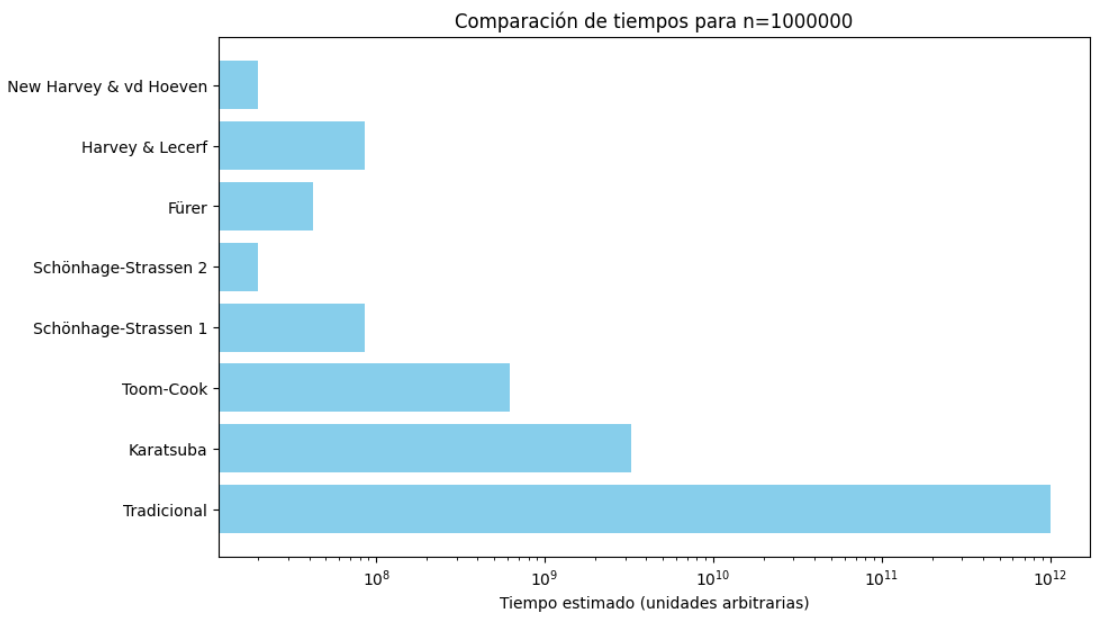
\includegraphics[scale=0.7]{figures/graficobarras.png}
    \caption{Gráfico de barras}
    \label{fig:chart_a}
\end{figure}


\paragraph{Análisis} 
El gráfico de barras permite comparar directamente el tiempo teórico que cada algoritmo requeriría para multiplicar dos enteros de un tamaño fijo. Se observa que los algoritmos clásicos, como la multiplicación tradicional (\(O(n^2)\)), presentan tiempos considerablemente mayores frente a métodos más avanzados como Karatsuba o Toom-Cook y estos a su vez presentan tiempos superiores a los presentes en New Harvey-van der Hoeven algorithm y Schönhage-Strassen second algorithm.

\clearpage

\subsubsection{Gráfico de tiempo vs tamaño de entrada}

\begin{figure}[!ht]
    \centering
    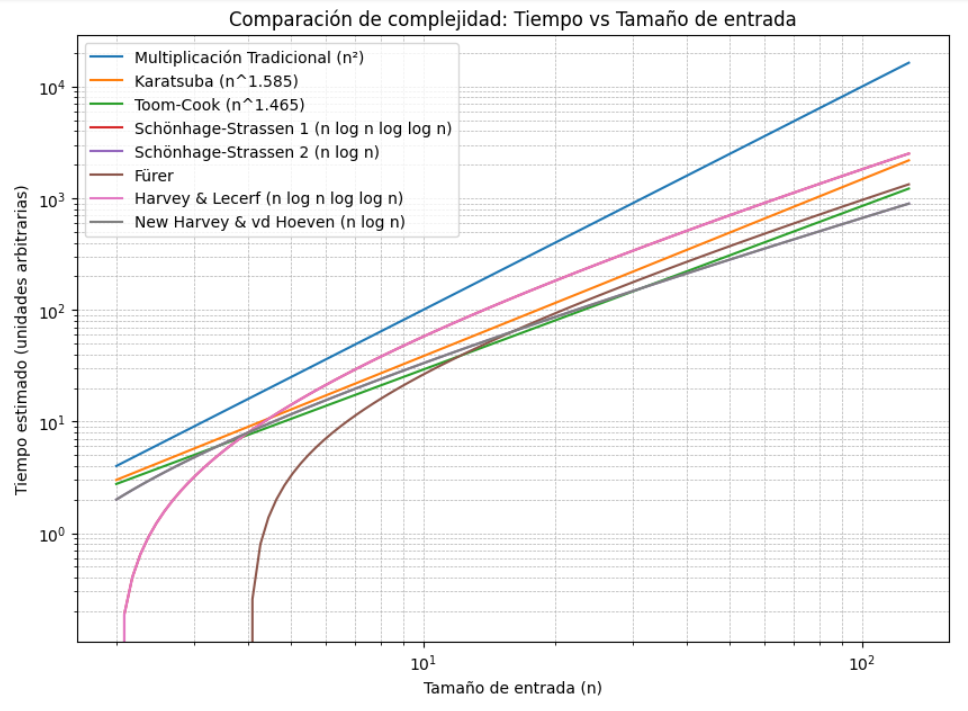
\includegraphics[scale=0.7]{figures/graficotvst.png}
    \caption{Gráfico de tiempo vs tamaño de entrada}
    \label{fig:chart_a}
\end{figure}

\paragraph{Análisis}
El gráfico de tiempo vs tamaño de entrada permite comparar directamente el tiempo teórico que cada algoritmo requeriría. Se observa que los algoritmos clásicos, como la multiplicación tradicional (\(O(n^2)\)), presentan un crecimiento prácticamente cuadrático. En contraste, los métodos más avanzados muestran un crecimiento más lento en el eje vertical (tiempo), lo que genera una curvatura visible que se acentúa a medida que mejora la complejidad algorítmica. Esta curvatura refleja cómo los algoritmos más eficientes escalan mejor con tamaños de entrada crecientes, ofreciendo un rendimiento teóricamente superior.

\clearpage

\subsubsection{Gráfico de caja}

\begin{figure}[!ht]
    \centering
    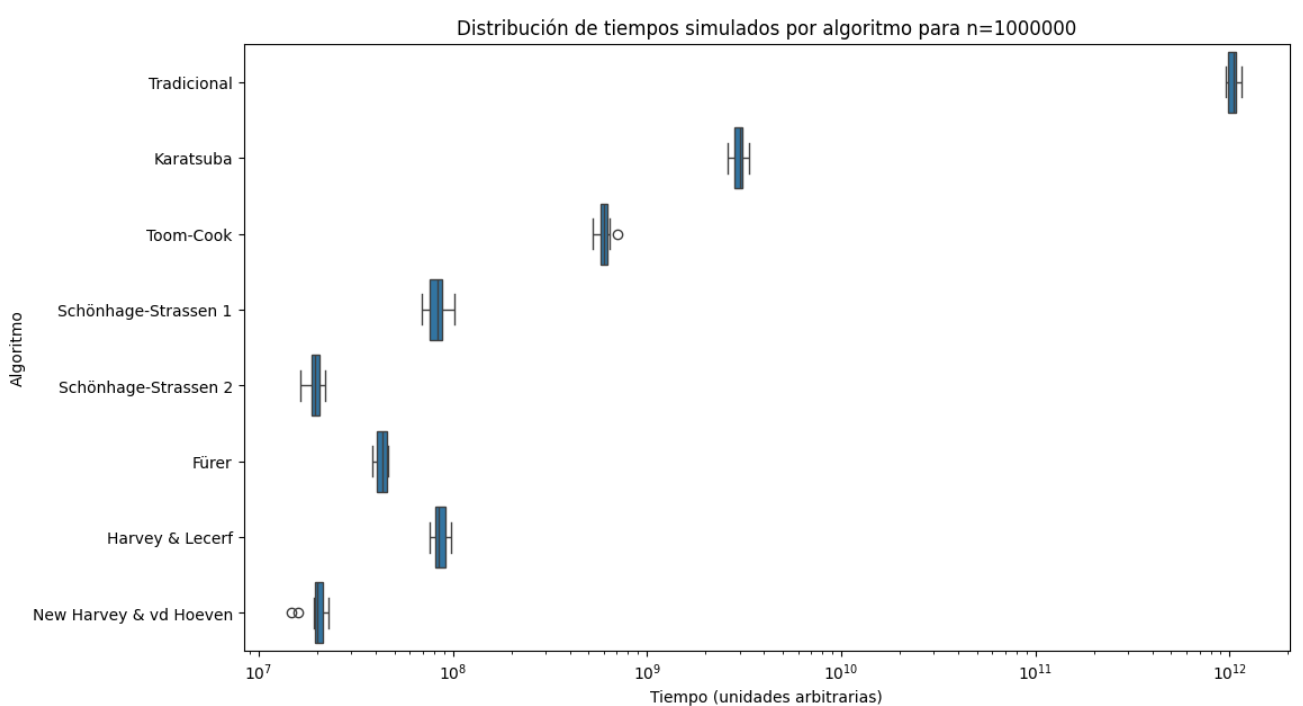
\includegraphics[scale=0.6]{figures/graficocajas.png}
    \caption{Gráfico de caja}
    \label{fig:chart_a}
\end{figure}

\paragraph{Análisis}
El gráfico de caja permite visualizar la variabilidad del tiempo teórico entre algoritmos en diferentes tamaños de entrada. Cada caja representa la distribución de tiempos para un algoritmo específico, permitiendo observar la mediana, los cuartiles y posibles valores atípicos. Se evidencia que los algoritmos con mayor complejidad, como la multiplicación tradicional, tienden a tener una dispersión más amplia a medida que el tamaño de entrada crece. En cambio, los algoritmos más eficientes presentan cajas más compactas, lo que indica una mayor estabilidad y menor variación teórica del tiempo de ejecución. Esta visualización resulta útil para comparar no solo el rendimiento promedio, sino también la consistencia de cada enfoque.
\clearpage

\section{Comparación general}

\paragraph{Complejidad asintótica} 
Los algoritmos muestran una evolución clara desde la multiplicación tradicional con complejidad cuadrática \( O(n^2) \), hasta algoritmos más avanzados como Karatsuba \( O(n^{1.585}) \), Toom-Cook \( O(n^{1.465}) \), y finalmente el algoritmo de Harvey–van der Hoeven con complejidad óptima \( O(n \log n) \). La tendencia decreciente dentro de la complejidad representa para nosotros avances significativos en eficiencia teórica.

\paragraph{Visualización de rendimiento} 
Los gráficos generados evidencian la diferencia en el crecimiento del tiempo teórico a medida que se incrementa el tamaño de entrada. Mientras que los algoritmos clásicos presentan curvas que crecen rápidamente, los algoritmos modernos muestran un crecimiento mucho más moderado.

\paragraph{Aplicabilidad práctica} 
Si bien algunos algoritmos modernos ofrecen mejor rendimiento teórico, su implementación puede ser más compleja y especializada. En la práctica, algoritmos como Karatsuba o Toom-Cook ofrecen una buena relación entre eficiencia y facilidad de implementación, siendo útiles para tamaños de entrada medianos.

    \input{chapters/05_discussion}
    \chapter{Conclusiones}
\label{ch:con}
\section{Conclusiones}

Este proyecto tuvo como propósito principal recapitular la evolución de los algoritmos de multiplicación de enteros, haciendo énfasis en el algoritmo propuesto por Harvey y van der Hoeven, primero en alcanzar una complejidad teórica óptima de \( O(n \log n) \).

A lo largo del trabajo, se revisaron los principales métodos que quedaron marcados en la historia del problema, comenzando con la multiplicación tradicional, pasando por Karatsuba, Toom-Cook y Schöhage–Strassen, hasta llegar al avance moderno representado por Harvey–van der Hoeven; planteando la idea principal y en esencia el concepto de cada uno acompañado de su complejidad computacional, con el fin de contextualizar cada uno dentro del hito que marcaron. Reafirmando que el aun nuevo algoritmo de Harvey y van der Hoeven presentado no hace mucho en el año 2020 no solo resuelve un problema abierto por décadas, sino que sienta las bases para futuras optimizaciones.

    \input{chapters/07_reflection}


    

    
    % -------------------------------------------------------------------
    % Bibliography/References  -  Harvard Style was used in this report
    % -------------------------------------------------------------------
    \bibliography{references}  %  Patashnik, O. (1988), BibTEXing. Documentation for general BibTEX users.
    
    % -------------------------------------------------------------------
    % Appendices
    % -------------------------------------------------------------------
    
    \begin{appendices}
        \input{chapters/appendix_A.tex}
        \input{chapters/appendix_B.tex}
    \end{appendices}
    
\end{document}
